\documentclass[letterpaper]{acm_proc_article-sp}
\usepackage{url}
\usepackage{listings}

%% Bring items closer together in list environments
% Prevent infinite loops
\let\Itemize =\itemize
\let\Enumerate =\enumerate
\let\Description =\description
% Zero the vertical spacing parameters
\def\Nospacing{\itemsep=0pt\topsep=0pt\partopsep=0pt\parskip=0pt\parsep=0pt}
% Redefine the environments in terms of the original values
\renewenvironment{itemize}{\Itemize\Nospacing}{\endlist}
\renewenvironment{enumerate}{\Enumerate\Nospacing}{\endlist}
\renewenvironment{description}{\Description\Nospacing}{\endlist}

% Disable the copyright and boilerplate for now
\makeatletter
\let\@copyrightspace\relax
\makeatother

\begin{document}
\lstset{
	language=Java,
	numbers=left,
	tabsize=2,
	showstringspaces=false,
	basicstyle=\ttfamily\small
}
\conferenceinfo{UWCSE503}{'10 Seattle, WA USA}

\title{JavaGrok: Automatic Inference of Documentation for Under-documented Code}

\numberofauthors{1} 
\author{
\alignauthor
Colin S. Gordon, Reto Conconi, Gilbert Bernstein, Michael Bayne\\
       \affaddr{University of Washington}\\
       \affaddr{Seattle, WA USA}\\
       \email{\{csgordon,conconir,gilbo,mdb\}@cs.washington.edu}
}

\maketitle
\begin{abstract}
Modern software development increasingly involves the use of third party
libraries. Developers now routinely locate and learn the APIs of myriad
libraries in the course of a single software development project. This process
is made more difficult by the fact that many libraries are poorly documented.
The developer often has to read the library source code or resort to trial and
error to determine how to correctly use the library. These methods of learning
about the library are time consuming and error prone.

We present a method to automatically augment library API documentation with invariants
inferred by a variety of static analyses. These include argument nullability,
argument and receiver mutation, argument leaking and capturing, and conditions
that will cause exceptions to be thrown.

We also perform a user study to
evaluate the usefulness of the additional documentation for developers.
\end{abstract}

% These categories are from the ACM CCS (Computing Classification System)
% http://portal.acm.org/ccs.cfm
\category{F.3.1}{Specifying and Verifying and Reasoning about
Programs}{Specification techniques}
\category{D.2.7}{Distribution, Maintenance, and Enhancement}{Documentation}
\category{D.2.13}{Software Engineering}{Reusable Software}

% These "terms" are from the ACM's official General Terms classifications.
% http://www.acm.org/about/class/1998
\terms{Documentation, Human Factors, Languages}

\keywords{Documentation Inference, Software Documentation, Static Analysis}

\section{Introduction}

Despite their best intentions, many developers routinely fail to provide
adequate or any documentation of the code they write.  Whether because of bad
practice, laziness or a sincere belief on the part of programmers that their
code will soon be thrown away, much code in regular use remains undocumented.
New developers join the team, the code is handed off to another group, or
perhaps even posted publicly on the Internet.  By various means, this code
finds its way into the hands of programmers who---having been assured that this
code will save them weeks of effort---now face a thoroughly unenviable task:
grok a lump of un(der)documented code and learn its interface well enough
to solve their original problem.

%Ideally, we would have an army of ingenious, classically trained Shakespearean
%typing monkeys, ready to provide high-quality documentation for all our
%programs and libraries at the drop of a hat.  However in reality, we, the
%unlucky developers often must make do with a single use case or oblique e-mail
%offering advice---if we get anything at all.  Sitting at our desks, we curse
%fate, the code in front of us, and the anonymous (or not so anonymous)
%programmer responsible for our pain.  We wonder, wouldn't it be nice if we
%could just push a button and get some useful, if not perfect documentation?

%We wonder, wouldn't it be nice if we could just push a button and get some useful, albeit imperfect documentation?
We believe it would be useful to have a tool that could generate partial
documentation of at least simple properties.

The prototype tool we describe here, JavaGrok, seeks to do just this.  By
applying static analyses to library source code and then
translating the results into human readable form, we are able to
automatically construct or augment Javadoc documentation.
Using this tool, we
consider the hypothesis that a significant amount of user pain and frustration
with un(der)documented libraries is due to confusion about
properties discoverable via static analyses. We consider analyses for nullability, mutability,
reference leaking and capturing, and exceptional conditions.
Here, we distinguish between confusions about formal properties
and conceptual
or higher level confusions about the proper way to use a library, focusing on
the formal properties.

To explore this hypothesis we conduct a user study, comparing developers'
experience using a poorly documented library with and without our
annotations.  We look at the participants' experience as revealed
by how frequently the
documentation fails to help resolve confusions, how frequently source
code is referred to instead of documentation, and via qualitative exit
questionnaires.  We plan to use this feedback to evaluate whether the augmented
documentation reduced developer confusion.

Although there has been some previous work on automatic
documentation annotation~\cite{autodoc}, this is the first user study
to directly address the question
``Is automatically generated documentation helpful?''
Previous work sought to answer the question
``Is automatically generated documentation accurate or more informative than
exemplar user documentation?''
While this question is certainly interesting in its own right,
we believe that determining whether the generated documentation is effective in aiding
developers to be a crucial question.

%Our hypothesis is that the properties and facts explained above help the 
%client of a library to accomplish a programming task in which the programmer
%has to use this library without any prior knowledge about it.
%In section~\ref{sec:Evaluation} we will discuss our results of our user study
%whether our hypothesis proved true.



\section{Example}
\label{sec:Example}

Consider Figure \ref{fig:pre}, a na\"ive collection object.
A programmer looking at the method interface of 
\texttt{public Object getAll()} does not know
that \texttt{getAll()} will leak a reference to its
internal representation. This might be surprising
if the list of objects that gets returned keeps growing
even though the caller of \texttt{getAll()} does not add those objects.

\begin{figure}[h]
\begin{lstlisting}
public class A
{
	private LinkedList<Object> list;
		
	public A() {
		list = new LinkedList<Object>();
	}
		
  public void add(Object o) {
   	list.add(o);
  }
    
	public List<Object> getAll() {
		return list;
  }
}
\end{lstlisting}
\caption{An example unannotated class.}
\label{fig:pre}
\end{figure}

But with information about reference leaks and captures added, a programmer can 
determine that she or he will not have an unique reference
to the list of all objects.  Knowing the reference is still shared by the
library, a developer may decide to copy the content 
of the list into a newly created list.  Figure \ref{fig:postannotation}
shows a class annotated with reference leak and capture information produced by
our tool.

\begin{figure}[h]
\begin{lstlisting}
public class A
{
	private LinkedList<Object> list;
	
	@UniqueReturn
	public A() {
		list = new LinkedList<Object>();
	}
		
  public void add(@Retained Object o) {
   	list.add(o);
  }
  
	@NonUniqueReturn
	public List<Object> getAll() {
		return list;
  }
}
\end{lstlisting}
\caption{An example class annotated with capture and leak information.}
\label{fig:postannotation}
\end{figure}

For a simple example such as this, inspecting the library code is not a
significant burden for the developer.  But as library size and complexity grow,
it is preferable to refer to condensed documentation rather than
deciphering library code.
Fortunately Javadoc will reproduce any source annotations in the HTML
documentation it produces.  For \texttt{getAll()}, the documentation will
include the annotations JavaGrok added.

\section{Analysis}

In this section we describe the analyses we perform: their implementation,
output, and why each analysis would be useful for a developer.

\subsection{Javarifier}
\label{sec:Javarifier}

Javarifier is a tool to infer reference immutability information built in
conjuction with research done by Quinonez et al.~\cite{Javarifier}. It infers
mutability constraints for object fields, method arguments and receivers. Those
constraints may be \texttt{mutable}, \texttt{readonly}, \texttt{?~readonly},
\texttt{polyread}, and \texttt{this-mutable}. The \texttt{?~readonly}
constraint indicates a method argument with a \texttt{readonly} upper bound and
a \texttt{mutable} lower bound. The \texttt{polyread} constraint provides
polymorphism over mutability for method arguments and receivers
(i.e. indicating that a method is read-only when called through a read-only
reference or mutable when called through a mutable reference). A
\texttt{this-mutable} reference provides similar polymorphism for object
fields: a \texttt{this-mutable} field is mutable if \texttt{this} is mutable
and read-only otherwise.

Javarifier produces its results directly in the JAIF format which allows us to
easily integrate it into our toolchain. We need simply to express the meaning
of its inferred constraints in the Javadoc documentation in concise language.

\subsection{Uno}

Uno is an open source tool which is the outcome of research done by Ma and
Foster~\cite{Uno}. It infers alias and encapsulation properties for Java.  The
tool generates annotations which provide information about how a certain
function treats its parameters, return values and fields (in the case of a
non-static function) when called. E.g. if a function captures or leaks a
reference or returns a new unique reference.

The tool generates annotations which are stored in a single separate file. 
To integrate the analysis results of UNO into the Java documentation we
use our own framework. We implemented a tree visitor inside the Java 7 
compiler that, at initialization, reads in the file generated by UNO and 
stores the information in a hashset. During the iteration over the AST
our visitor inserts annotation at the appropriate places.

Our tool will annotate methods with the information if the method returns a 
unique reference (that means a reference to an object that is not referenced 
by any other reference). We think that this information is helpful to the 
programmer because we think it is curcial to now if one is the sole owner of 
an object or not. For a example considering a list object. If one is the sole
owner of the list then one can be sure that after adding an element to the list
and calling a method somewhere in a library the list is guaranteed to still 
contain exactly one elment, because the list was not reachable from anywhere
else.

Furthermore JavaGrok also documents parameters and tells the client
of those functions if a previously unique reference is still unique after the 
called method to which the object was passed as an argument. Analogously to 
above, this information is useful to find out if one is still the sole owner
when one passes a unique reference to a method. Based on our own experience
as programmers we think that knowing such facts helps preventing bugs.

\subsection{Thrown Exceptions}

Java requires that checked exceptions be declared by methods that raise them,
but it unfortunately cannot require that they be well documented, and
frequently the conditions under which exceptions are raised are unclear to a
library user. Even with checked exceptions, often a supertype of a thrown
exception is declared.  While knowing that an \texttt{IOException} might be
thrown is useful, knowing that the method might throw either a
\texttt{FileNotFoundException} or \texttt{InterruptedByTimeoutException} is more
useful to a developer, because knowing the specific exception may help to debug
a program.  Additionally, unchecked exceptions need not be declared in Java method
signatures or documentation and can remain entirely invisible to the library
user until they are encountered at runtime.

To alleviate this, we infer some of the conditions under which a method would
throw an exception, and produce annotations of the form:

\begin{verbatim}
@ExceptionProperty(throwsWhen =
    "{IllegalArgumentException} when (x < 0)")
public Object getElement(int x) { ... }
\end{verbatim}

This sort of inferred information can inform developers of unchecked exceptions,
and alert them to otherwise undocumented assumptions of a library without
requiring developers to dig through the library's code.
Annotations may contain a list of exceptions and conditions, and for some
complex conditions we reduce the condition to ``sometimes'' because our analysis
is purely syntactic.  We do not use an
existing analysis tool because none were available for this task, but even our
syntactic analysis provides useful results.

Our analysis is a fairly simple search for explicit throws, tracking branch
statements at the purely syntactic level on the
way to such statements.  We propagate information about exceptional conditions
between methods by purely syntactic replacement of formal arguments by actual
arguments.  We do not account for intermediate side effects on variables, or
track data flow from arguments to local variables or object fields.  In
practice, we have not found this lack of precision to be problematic as most of
the thrown exceptions we see are from argument validation.

Buse and Weimer infer documentation for exception conditions
using an analysis performs that some symbolic execution along paths to reach throw
statements, propagating information between methods as necessary~\cite{autodoc}.
Because they
perform full symbolic execution, their tool can be much more precise than ours.
Replacing our exception analysis with theirs, or implementing our own symbolic
execution would likely improve the quality of our exception documentation.  

As in Buse and Weimer's work, we expose internal field names and
local variable names in exceptional conditions.  We agree with their assessment
that while this leaks some
implementation information and is not necessarily informative, in practice
leaked variables are still useful: for example, showing that an exception is
thrown from a list's \texttt{remove()} method when a local variable \texttt{len}
is equal to 0 has clear implications.

\subsection{Nullability}
\label{sec:Nullability}

In heavily object oriented languages like java, every variable is nullable
(aka. option, maybe), capable of holding either a reference to a value or the
special value null.  Because of this ubiquity, one common mistake is to call
methods with null parameters they are unprepared to handle, or to erroneously
assume that returned values are never null.  Well documented libraries, like
the Java collections framework, will frequently spell out when variables are
assumed to be nullable or not-null when an ambiguity seems likely.

By means of a nullability inference~\cite{NIT,NonNullTypeInference} we can add
similarly useful type decorations to documentation.  Although two Java
nullability inferences are freely available, they are both whole program
analyses and therefore ill-suited to our target application: library
documentation.  We plan to first try adapting their existing analysis code, or
failing that re-implement a modular version of their analysis within our own
framework.



\section{Technical Approach}
To infer information about Java code we use existing Java inference tools and 
combine their output. Additionally we have our own framework which allows us to
implement our own analysis. 

To combine all analysis tools (including our own ones) we have to bring 
their results into a common format at some point in our toolchain. 
We will use the JAIF (Java Annotation Index File) format as our common format. 
Firstly because the Javarifier tool generates its output in this file format. 
Secondly because there do exist tools which allow to extract annotations from 
annoted byte code. This makes it easy to use existing tools which embed their 
results into the byte code.

\begin{figure}
\centering
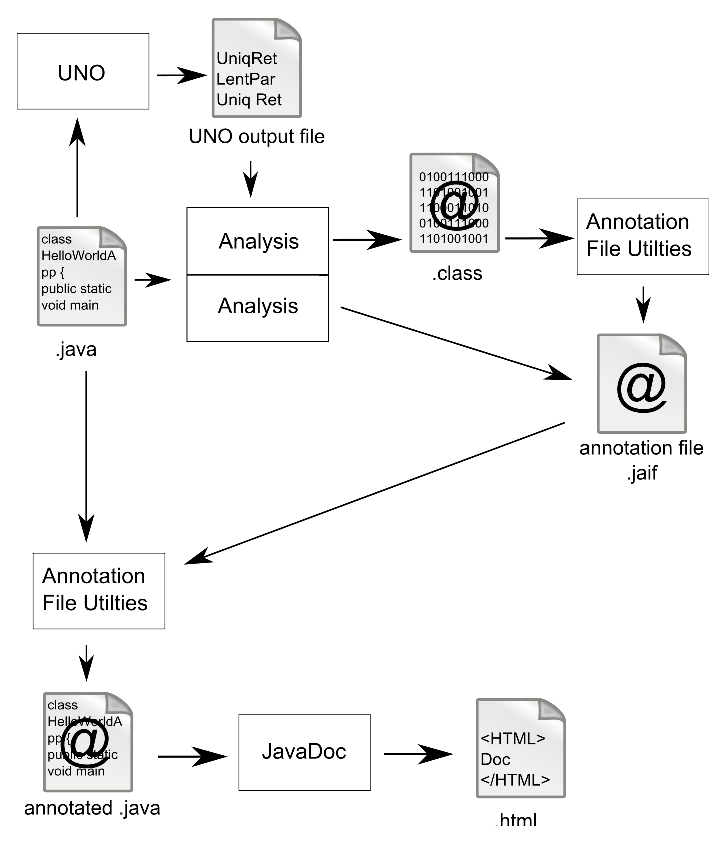
\psfig{file=figures/technicalApproach/technicalApproach.eps, width=2.1in}
\caption{Toolchain}
\label{fig:toolchain}
\end{figure}

\subsection{Analysis Framework}
\label{ss:analysisFramework}

To implement our own analysis tools we use the current version of the Java 7 compiler.
This allows us to use it's plugin architecture to write our own analyzers. From within
a Java compiler plugin we can access the compiler's abstract syntax tree and we can emit 
annotation to the class files. As described above those annotation will get extracted 
with the annotation file utilities.

In the sections~\ref{sec:Javarifier} until~\ref{sec:Nullability} we show how each analysis 
generates information and transforms it's result to the JAIF format.

\subsection{Javarifier}
\label{sec:Javarifier}
TODO Michael


\subsection{Uno}

Uno is an open source tool which is the outcome of a research work done by
Ma and Foster~\cite{Uno}. It infers alias and encapsulation properties for Java.
The tool generates annotations which provide information about how a certain function
treats it's parameters, return objects and fields (in case of a non-static function) 
when called. E.g. if a function captures or leaks a reference or returns a new 
unique reference.

The tool generates annotations which are stored in a single seperate file. We plan
to either change the output mechanism of the tool in a way that it directly generates
JAI files or to write a rewriter which transforms files from Uno's file format to the
JAIF format.

In case we realise that the tool is not fulfilling our needs

\subsection{Precondition/Dependency}

TODO Colin

\subsection{Nullability}
\label{sec:Nullability}
TODO Gilbert


\subsection{From JAIF to HTML documentation}

To get the inferred information back into the source files we use the annotation 
file utilities (\cite{AFU} AFU). The next step is to run JavaDoc over our
annotated source code. A JavaDoc plugin (called doclet) is needed which will
cause JavaDoc to generate documentation for our new annotations. The output will
generate a HTML documentation of the code enriched with automatically inferred
properties expressed in a programmer friendly format.

Figure \ref{fig:toolchain} shows the stages in our toolchain.

\section{Evaluation} \label{sec:Evaluation}
We performed a small experiment wherein developers were given a third party
library and a set of programming tasks. They were asked to report on certain
events that occurred while completing the tasks. We specifically focused on
when the developer had questions about how to correctly use the library, and
considered four cases: a) the question was answered by our annotations, b) the
question was answered by the existing library documentation, c) the question
was answered by reading the library source code, and d) the question was not
answered. We also asked the developers to note any time they were surprised by
the library's behavior.

Our hypothesis was that by augmenting library documentation with inferred
properties, we would decrease the frequency with which developers needed to
refer to the library source code to answer questions. This would show up as a
non-zero incidence of questions being answered by annotations and a
corresponding decrease in the questions that were answered by reading source
code. We also hypothesized that our annotations may have resulted in a
reduction in surprise at library behavior, and would not increase the incidence
of surprise.

\begin{figure*}
\centering
\begin{tabular}{ l | r r r r | r }
 & \multicolumn{4}{| c | }{Question answered by:} & \\
Developer & Annotations & Docs & Source & Unanswered & Surprised \\
\hline
Dev 1 & 0 & 14 & 0 & 1 & 0 \\
Dev 2 & 1 &  5 & 2 & 1 & 0 \\
Dev 3 & 1 &  3 & 0 & 0 & 0 \\
Dev 4 & 1 &  6 & 1 & 1 & 0 \\
\hline
\textit{Experiment} & 3 & 28 & 3 & 3 & 0 \\
\hline
Dev 5 & - &  4 & 0 & 0 & 0 \\
Dev 6 & - & 13 & 2 & 3 & 1 \\
Dev 7 & - & 10 & 0 & 2 & 0 \\
Dev 8 & - &  7 & 1 & 2 & 1 \\
\hline
\textit{Control} & - & 34 & 3 & 7 & 2 \\
\hline
\end{tabular}
\caption{Experiment Results}
\label{fig:exp_results}
\end{figure*}

\subsection{Experiment Design}
The experiment involved two groups of four developers each, all of whom were
University of Washington computer science graduate students. The developers
were given a set of programming tasks involving the creation of simple
interactive animations. They were supplied with the Nenya~\cite{nenya} graphics
and animation library to use to complete those taks. None of the developers had
previously seen or used the library. The experimental group was provided with
augmented documentation and source code for the library, and the control group
was provided with original, unmodified documentation and source code.

There were four tasks that were designed to be completable within a single
hour. Developers were told that they were free to leave after one hour, even if
they had not completed all of the tasks.

The members of each group were provided with the Eclipse IDE, configured to
provide ready access to the appropriate documentation and source code. As the
subjects' experience with the Eclipse IDE was quite varied, they were shown how
to access both the library documentation and source code. The aim was to reduce
the likelihood that differing familiarity with the IDE would influence their
decision to inspect the documentation or source.

The subjects were instructed to first check the documentation when they
encountered a question about correct usage of the library, then to consult the
source code only if their question was not answered to their satisfaction by
the documentation. Finally they were asked to record the outcome of each event.
The experimenter could record a question as being resolved by ``annotations'',
``documentation'', ``source code'' and ``not resolved''. The control group had
only the latter three choices as they had unaugmented documentation.

We also instructed subjects to complete a short survey after finishing the
experimental tasks. The results of this survey were not intended to directly
validate or refute our hypothesis, but to help us to gauge other aspects of the
work, better understand ambiguous results, and to direct future work. Data from
the survey are mentioned in the discussion below. The results of our experiment
are shown in Figure ~\ref{fig:exp_results}.

\subsection{Discussion}
We knew we had a small test group, so we were looking for a striking difference
between the control and experimental groups.  The results had no such strong
trends, rather they were inconclusive.  Our sample size of developers was not
large enough to be statistically significant, but the developer surveys exhibit
a mixture of both positive and negative trends.

Most developer complaints from both the experimental and control groups were
about the high-level usage model of the library being unclear.  This suggests
the evaluation task was
a poor choice for evaluating our tool; our tool infers small technical
properties of the code, not use models for the library.  A better task would
have required use of our annotations or close source inspection to avoid some
subtle bugs.  Only the control group ever said they were surprised by library
behavior, but the surprises were about higher-level component interactions such
as what order to call a pair of methods, not about properties JavaGrok can
infer.

None of the developers in the experimental group found the annotations to be
frequently useful.  None answered more than one question using the
annotations, which was never more than 1/9th of a subject's questions.  Most
questions for both groups were answered by reading the existing documentation.

There was however some positive feedback from the experimental group.  All
found the annotations to be of a useful level of detail, and 3 of 4 said they
considered the annotations
to be potentially useful, but not for the evaluation task.  This generally
positive response reinforces our belief that the properties
JavaGrok infers could be useful.  It is also possible that other properties
exist that could have been inferred and would have been useful for our chosen
evaluation task.

In designing
our experimental task, we struggled to find a balance between designing a
realistic task, and designing a task geared towards requiring annotations.  We
settled on a task we felt was reasonably general and might benefit from the
generated annotations.  Designing a task specifically to make the annotations useful would
not have helped us understand how useful they were generally, but the situations
where they would provide benefit seem not appear to occur in such a short exercise.
Upon reflection, we suspect that the target experiment time of one hour per
subject, chosen to encourage volunteers, may simply not be enough time to run
into tricky cases where the very particular information JavaGrok documents would
be useful.  We suspect that the annotations might prove valuable in a longer
study, using a library over a longer period of time, allowing more time to run
into what we acknowledge are usually corner cases where specific information
about JavaGrok's properties would prove useful.  One of our subjects said he
suspects they may prove more useful in debugging than in development.

While our actual results showed no significant benefit to JavaGrok's annotations
for this task, the generally positive response to the idea from our test
subjects suggests that automatically inferred documentation deserves more
thorough study.



\section{Related Work}
There is a wealth of work on inferring interesting properties of existing code,
but most of these are focused on inferring properties suitable for checking.
Because our goal is not to prove absence of errors, but to simply infer correct
information that is useful to the developer, some flexibility is available to us
that is not possible for much of that work.

The most directly relevant work is Buse and Weimer's system for automatically
inferring documentation for conditions that will result in a Java method
throwing an exception~\cite{autodoc}.  We use a modification of their
algorithm, and also perform several other analyses to provide a broader range
of information.

\subsection{Individual Analyses}
Some text for nullability.

Quinonez, et al.~\cite{Javarifier} described a technique for inference of
reference immutability in Java and implemented it in a tool called {\sc
  Javarifier}. Their goal is the inference of annotations for the {\sc Javari}
language (an extension of Java) which enforces reference immutability
constraints. TODO: IGJ~\cite{IGJ}, Pidasa~\cite{Pidasa}.

Cherem and Rugina~\cite{UniquenessInference} inferred uniqueness using a two-level
abstraction. A intraprocedural analysis which is flow-sensitive and an interprocedural
one that is flow-insensitive. Combined they get uniqueness information
which is used to actively free Java object whenever an unique reference gets lost.

Aldrich, Kostadinov and Chambers~\cite{AliasJava} showed how alias information 
helps the programmer to understand how data is shared in large software systems.

Buse and Weimer~\cite{autodoc} automatically infer documentation for
exceptions, and the exception analysis in our work is directly based on the
refined version of {\sc Jex} [citation needed] they present.


\section{Conclusion}

The results of our user evaluation were inconclusive.  We did not reach any
reliable conclusion on whether JavaGrok's annotations are helpful to programmers
in practice.  There are a number of possible reasons our study was ineffective.

First and most significantly, we found it very difficult to pick a suitable
task.  We rejected many tasks because they were too simple.  These tasks did not
appear likely to benefit from documentation of the properties JavaGrok infers.
On the other hand, the tasks we did choose were complex and difficult, but primarily due
to a lack of informal, high level documentation.  The formal properties that
JavaGrok inferred proved to be mostly irrelevant for what subjects were asked to
do.

When we began this project, we chose to find and use pre-existing analyses in
order to save time.  In hindsight, this was a questionable choice.  The analyses
were surprisingly difficult to get working and integrated together.  Once the
analyses were integrated and ran, we found that the results were somewhat
ill-suited to our documentation purposes (e.g. the lack of \texttt{@Nullable}
annotations noted by one of our test subjects). We now believe that creating
analyses tailored to documentation generation is a promising and possibly more effective
approach.

However, most experimental group test subjects thought the generated annotations would be
useful.  This leads us to believe that the principal failing of our experimental
design was a poor choice of developer task.  A better task could take two forms.  A more carefully
selected or specially engineered task could be used to test the negative
hypothesis:  Automatically generated documentation annotations are not useful in
a wide variety of situations and tasks.  If JavaGrok fails to help users
understand optimistically selected use-cases, we can conclude that it is
unlikely to help users at all.  However, demonstrating the positive hypothesis
will likely be more difficult.  For realistic programming tasks the annotations
may only be useful once in every fifty times a developer refers to the
documentation.  For this reason we believe that a longer a longer in-situ
industrial study is necessary to provide meaningful positive conclusions.



%ACKNOWLEDGMENTS are optional
\section{Acknowledgments}
The authors are grateful for the assistance of their volunteer user study
subjects.

\bibliographystyle{abbrv}
\bibliography{javagrok}

\end{document}
